\chapter{Materiali e metodi}
Il presente capitolo ha lo scopo di fornire tutto un insieme di informazioni preliminari utili a comprendere meglio i capitoli successivi, i quali rappresentano il vero corpo di questo lavoro di tesi. Innanzitutto viene presentata un'introduzione all'acquisizione di immagini radiografiche e alla tomografia computerizzata, mettendo in luce le differenze tra due tecniche fondate entrambe sull'attenuazione di raggi X da parte dei tessuti del corpo, ma nonostante ciò profondamente diverse. Successivamente vengono riportate in breve le basi teoriche della segmentazione e delle reti neurali impiegate nella segmentazione automatica. Infine si passa all'esposizione dei principali metodi statistici impiegati negli studi utilizzati per questa tesi.

\section{Formazione di un'immagine a raggi X}
La formazione di un'immagine a raggi X è la conseguenza dell'attenuazione di un fascio di raggi X a carico dell'oggetto investito dal fascio stesso. Come illustrato nella \figref{fig:apparatox}, sia prima sia dopo l'oggetto da indagare sono posti dei collimatori, in modo tale che i fotoni che arrivano sulla lastra siano sono quelli perpendicolari alla lastra stessa, dove si formerà l'immagine finale. L'attenuazione del fascio è maggiore per i tessuti duri e minore per i tessuti molli, mentre è quasi nulla per l'aria, come mostrato nella \figref{fig:radiografia}. L'attenuazione del fascio segue la legge di Lambert-Beer:
\begin{equation}\label{lambert}
    I(x) = I_0\,\mathrm{e}^{-\mu_\mathrm{l}x}\,,
\end{equation}
dove $I_0$ è l'intensità iniziale del fascio, \textit{x} è la coordinata spaziale che quantifica la distanza percorsa da un fotone all'interno di un certo materiale, e $\mu_\mathrm{l}$ è il coefficiente di attenuazione lineare del materiale per un'energia fissata del fotone. Nel caso di un fascio monocromatico emesso con intensità $I_0$ ed energia \textit{E}, che attraversa lo spessore \textit{x} di un corpo, si definisce la trasmittanza del fascio stesso come:
\begin{equation}
    T = \frac{I(x)}{I_0} = \mathrm{e}^{-\int_0^x \mu_\mathrm{l}(E,x')\,\mathrm{d}x'}\,,
\end{equation}
in cui è importante sottolineare che il coefficiente di attenuazione lineare $\mu_\mathrm{l}$ è funzione non solo dell'energia ma anche della posizione, in quanto la composizione del corpo investito dal fascio può essere varia. Inoltre, il coefficiente di attenuazione lineare dipende dal numero di massa atomica del materiale, dalla sua densità e anche dall'energia del fascio di raggi X, come si può osservare nella \figref{fig:trasmittanza}; si può dedurre che il coefficiente di attenuazione è proporzionale alla densità del materiale e inversamente proporzionale all'energia del fascio.
\begin{figure}[htp]
\centering
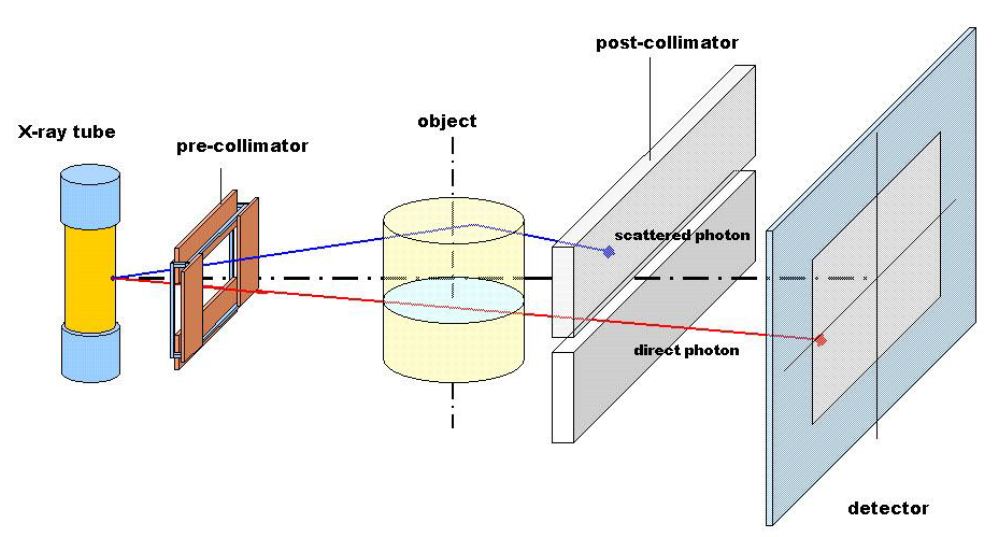
\includegraphics[scale=0.6]{Immagini/apparatox.png}
\caption{\label{fig:apparatox} \textit{Schematizzazione di un sistema per la formazione di immagini a raggi X}.}
\end{figure}
\begin{figure}[H]
\centering
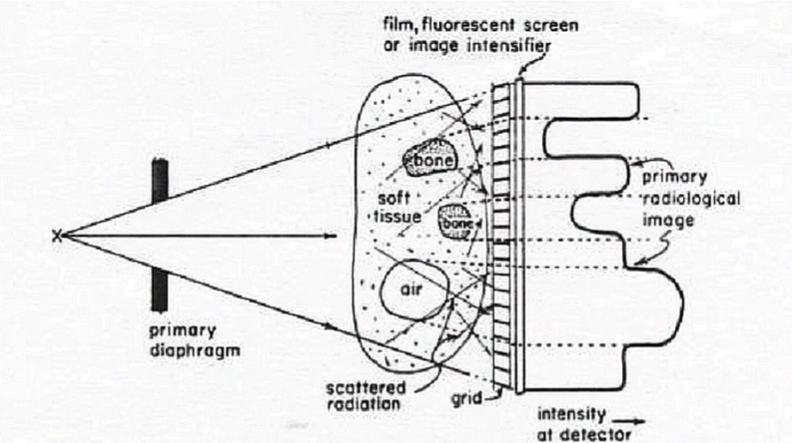
\includegraphics[scale=0.7]{Immagini/radiografia.png}
\caption{\label{fig:radiografia} \textit{Schema basilare per la formazione di immagini a raggi X}.}
\end{figure}
\begin{figure}[H]
\centering
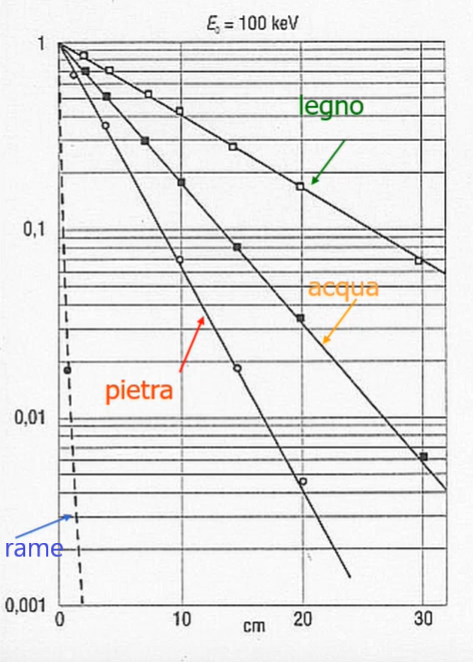
\includegraphics[scale=0.444]{Immagini/trasmittanza.png}\quad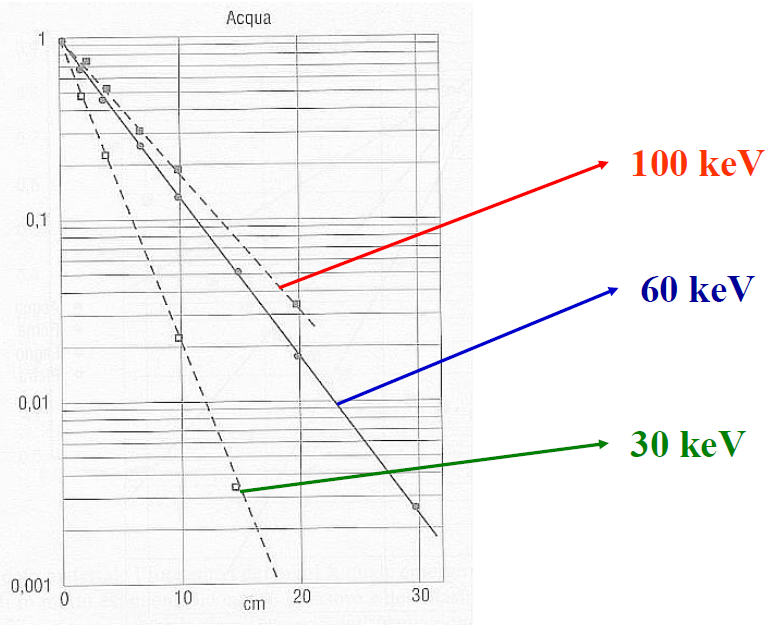
\includegraphics[scale=0.59]{Immagini/trasmittanza2.png}
\caption{\label{fig:trasmittanza} \textit{Da sinistra a destra: andamento della trasmittanza per materiali diversi a energia fissata e per energie diverse a materiale fissato}.}
\end{figure}

La dipendenza di $\mu_\mathrm{l}$ dai diversi parametri può essere espressa in funzione del coefficiente di attenuazione atomico $\mu_\mathrm{a}$ nel modo seguente:
\begin{equation}
    \mu_\mathrm{l} = \frac{\rho \mathrm{N_A}}{A} \mu_\mathrm{a}\,,
\end{equation}
dove $\rho$ rappresenta la densità del materiale, \textit{A} il numero di massa atomica degli atomi che lo compongono e $\mathrm{N_A}$ il numero di Avogadro.
Il coefficiente di attenuazione atomico ha le dimensioni di una sezione d'urto e indica la probabilità di interazione tra un fotone attraversante una superficie unitaria contenente un solo atomo e quest'ultimo. Per fotoni con energia non troppo elevata (inferiore a 1\,MeV) le interazioni con la materia possono produrre tre fenomeni distinti.
\begin{description}
    \item[Effetto fotoelettrico] È la conseguenza dell'assorbimento della radiazione da parte di un elettrone, che riceve l'energia sufficiente per sfuggire dall'atomo. L'energia della radiazione viene utilizzata in parte per rompere il legame fra l'elettrone e il nucleo, mentre la restante parte si trasforma in energia cinetica dell'elettrone.
    \item[\textit{Scattering} Compton] Si ha quando il fotone interagisce con un elettrone posto in un guscio esterno dell'atomo. Il fotone colpisce l'elettrone in un urto anelastico e viene deviato, fornendo all'elettrone l'energia necessaria per poter sfuggire dall'atomo.
    \item[\textit{Scattering} Rayleigh] In questo caso, l'urto fra il fotone e l'elettrone è elastico, di conseguenza non si ha trasferimento di energia, ma l'unico effetto che si osserva è una deviazione nella traiettoria del fotone.
\end{description}
Il coefficiente di attenuazione atomico si può scrivere come somma delle sezioni d'urto dei singoli fenomeni appena elencati, posti in ordine:
\begin{equation}
    \mu_\mathrm{a} = \tau + \sigma_\mathrm{C} + \sigma_\mathrm{R}\,.
\end{equation}
In medicina non viene utilizzata radiazione con energia superiore a 1,02\,MeV, poiché un fotone del genere, interagendo con un campo elettrostatico, avrebbe energia sufficiente per produrre una coppia elettrone-positrone. La predominanza di un fenomeno rispetto a un altro dipende sia dal numero atomico del mezzo sia dall'energia del fotone, come si può osservare nella \figref{fig:effetti}: l'effetto fotoelettrico domina a bassa energia e grande numero atomico, l'effetto Compton prevale a energie medie e tendenzialmente a numero atomico piccolo, mentre la produzione di coppie elettrone-positrone si osserva per alte energie e grande numero atomico.

\begin{figure}[htp]
\centering
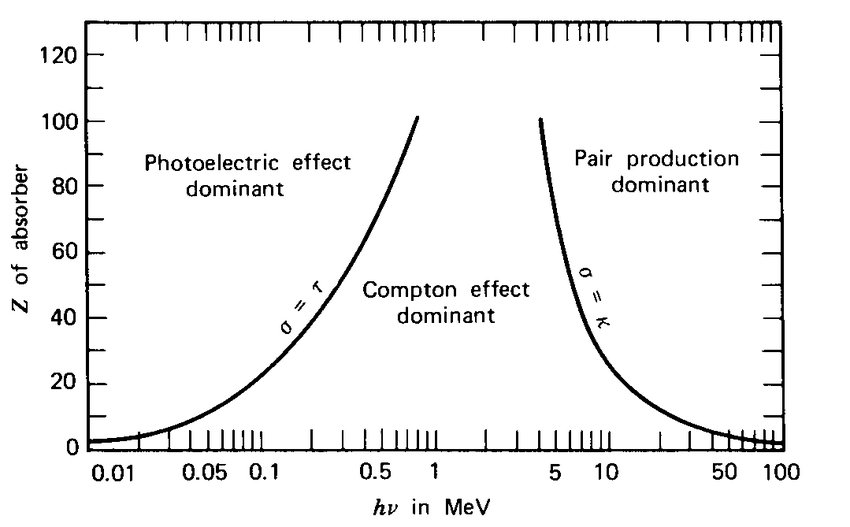
\includegraphics[scale=0.45]{Immagini/effetti.png}
\caption{\label{fig:effetti} \textit{Effetto prevalente in funzione del numero atomico del materiale e dell'energia della radiazione}.}
\end{figure}

\section{Tomografia computerizzata}
Inizialmente, con la \textbf{tomografia computerizzata} (TC) era possibile ottenere solo immagini tomografiche del piano assiale dell'organismo: per questo motivo era chiamata, e spesso lo è tuttora, tomografia assiale computerizzata (TAC), sebbene il nome corretto attualmente sia solo tomografia computerizzata.

La differenza fondamentale tra radiografia e tomografia è che la seconda è frutto di un ricalcolo e di una ridistribuzione del segnale nelle tre dimensioni, che non ha, quindi, lo scopo unico di fornire immagini radiologiche tridimensionali (tomografiche), ma riesce anche a mettere in evidenza dettagli che altrimenti non sarebbe possibile notare da una semplice serie di immagini radiografiche bidimensionali. Un'altra differenza fondamentale è il passaggio dal pixel al voxel, il che risolve le ambiguità dovute alla sovrapposizione di diversi oggetti lungo una direzione, non distinguibili in radiografia.

Il principio di ricostruzione dell'immagine nella TC è piuttosto semplice: si tratta di acquisire immagini radiografiche da direzioni diverse e metterle insieme per individuare il punto nello spazio in cui è collocato l'oggetto che ha generato l'attenuazione. Il numero di direzioni da acquisire si fonda su una regola empirica e dipende dalla risoluzione in pixel del rivelatore: il numero di direzioni di acquisizione deve essere comparabile al numero di pixel per riga del rivelatore. È inutile, perciò, acquisire un'immagine per ogni grado di angolo se si hanno, per esempio, solo 100 pixel per riga. Sebbene il coefficiente di attenuazione lineare che compare nella \eqref{lambert} dipenda sia dall'energia del fascio sia dalla densità del corpo investito, nella ricostruzione delle immagini di TC classica è spesso accettabile considerare $\mu_\mathrm{l}$ come funzione solo della densità. Ciò detto, prendendo come riferimento la \figref{fig:attenuazione}, la legge di Lambert-Beer diventa la seguente:
\begin{equation}
    I(x,y) = I_0(x,y)\,\mathrm{e}^{-\int\limits_L \mu_\mathrm{l} (x,y)\,\mathrm{d}l}\,.
\end{equation}

\begin{figure}[htp]
\centering
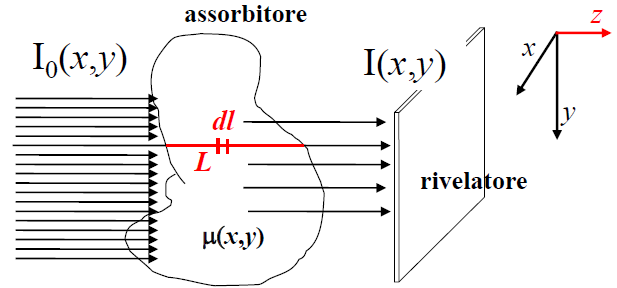
\includegraphics[scale=0.85]{Immagini/attenuazione.png}
\caption{\label{fig:attenuazione} \textit{Schematizzazione di una radiografia}.}
\end{figure}

\noindent Per ricostruire l'immagine bisogna recuperare i valori che assume il coefficiente di attenuazione lineare lungo \textit{L}; dunque, la singola radiografia è l'integrale della funzione $\mu_\mathrm{l}(x,y)$ lungo la direzione dei raggi X:
\begin{equation}\label{integralemu}
    \ln{ \left[ \frac{I(x,y)}{I_0(x,y)} \right]} = -\int\limits_L \mu_\mathrm{l} (x,y)\,\mathrm{d}l\,.
\end{equation}
A questo punto, acquisendo un'immagine con un rivelatore digitale non si ottiene un'immagine radiografica come quella delle lastre, con gli oggetti più attenuanti mostrati in bianco, bensì un'immagine dove i fotoni conteggiati vengono codificati in bianco e gli oggetti attenuanti in nero (o, per meglio dire, assenza di bianco). Da un'immagine del genere è impossibile ricavare l'integrale dell'\eqref{integralemu}, che invece si ottiene dividendo il valore d'intensità del fascio rivelato nell'immagine radiografica per il valore iniziale dell'intensità $I_0$ del fascio, che si può ottenere acquisendo un'immagine radiografica di campo vuoto; a questo rapporto si applica il logaritmo naturale. Il risultato è quello della \figref{fig:globo}, che mostra le immagini radiografiche iniziale e finale di un globo di legno. Osservando attentamente l'immagine, ad esempio nella zona in cui è presente il chiodo fra il globo e il telaio, si può vedere come l'operazione descritta dall'\eqref{integralemu} non ha il solo scopo di invertire i colori, ma ha soprattutto il compito di generare un contrasto corretto; in altre parole, se nella radiografia attenuata si è certi che due oggetti, di cui uno di gran lunga più denso dell'altro, venga riportato con il contrasto che effettivamente dovrebbe avere, nella radiografia acquisita questa certezza non c'è. L'operazione appena descritta non si può eseguire con un sistema classico di diretta incidenza dei raggi X sulla lastra.

\begin{figure}[htp]
\centering
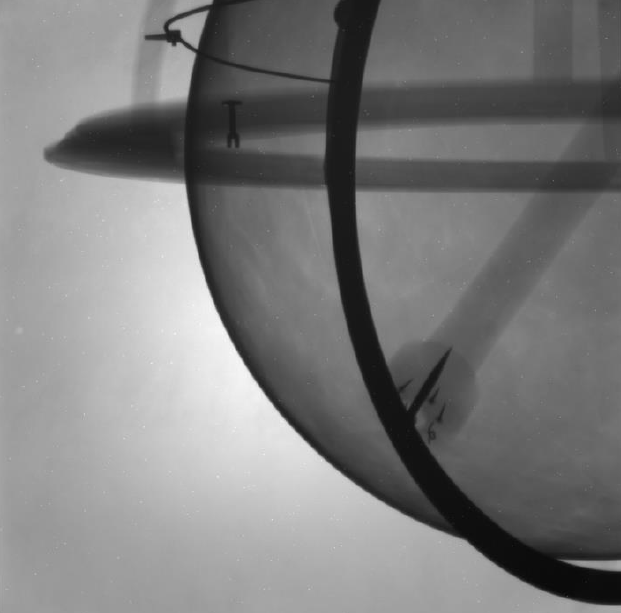
\includegraphics[scale=0.58]{Immagini/globo1.png}\quad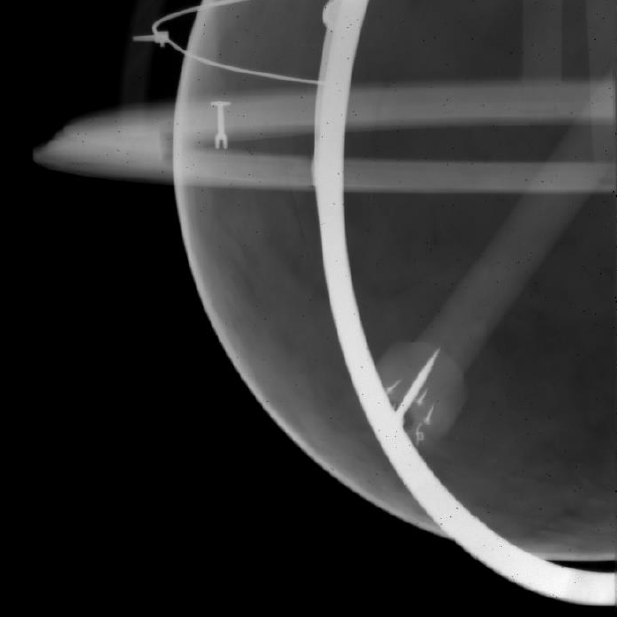
\includegraphics[scale=0.577]{Immagini/globo2.png}
\caption{\label{fig:globo} \textit{Radiografie acquisita e attenuata di un globo di legno}.}
\end{figure}

Nell'acquisizione di un'immagine radiografica è necessario anche eliminare il rumore, che appare con dei tipici puntini neri distribuiti casualmente in tutta l'immagine. Questi puntini sono dovuti a singoli raggi X che riescono a oltrepassare l'oggetto da esaminare senza interagire con esso e oltrepassano anche il rivelatore senza essere fermati, di conseguenza interagiscono direttamente con l'elettronica e vengono codificati con un'intensità estremamente elevata. Il rumore può essere eliminato con dei filtri locali, cioè metodi matematici di riduzione del rumore che prevedono la moltiplicazione dei valori d'intensità rilevata della matrice di pixel attorno a un punto per i valori di un'altra matrice detta \textit{kernel}. In pratica, si sovrappone il \textit{kernel} alla matrice dei pixel, si moltiplicano singolarmente le caselle della matrice dei pixel per le corrispondenti caselle del \textit{kernel} e si sommano tutti i valori della matrice risultante; il risultato rappresenta il valore d'intensità da assegnare al pixel al centro della matrice finale. L'operazione va ripetuta per ciascun pixel dell'immagine, attorno al quale si prenderà una certa matrice da moltiplicare sempre per lo stesso \textit{kernel}. Esistono diversi tipi di filtri, ognuno col suo \textit{kernel}, non solo per diminuire il rumore, ma anche per mettere in evidenza solo i bordi degli oggetti raffigurati nella radiografia, tralasciando l'immagine interna ai bordi qualora non sia utile, e anche per mettere a fuoco le immagini.

Ognuno di questi filtri, in realtà, sebbene riesca anche a risolvere il problema per il quale è stato impiegato, introduce sempre un qualche altro tipo di problema di piccola o grande entità. Per fare un esempio, un filtro per la riduzione del rumore tende ad individuare come rumore, e quindi anche a sopprimere, del segnale che in realtà non è rumore ma appartiene ai bordi degli oggetti visualizzati nell'immagine. Si tratta, perciò, di trovare dei compromessi in modo da applicare filtri che risolvano il problema senza introdurre altri difetti di entità troppo grande.

Il problema tomografico è, dal punto di vista matematico, un problema inverso, che prevede cioè la ricostruzione di un volume a partire da delle proiezioni radiografiche a diversi angoli. La soluzione dipende dai seguenti fattori:
\begin{itemize}[label=$-$]
    \item caratteristiche della sorgente;
    \item caratteristiche del rivelatore;
    \item geometria di acquisizione;
    \item numero di angoli.
\end{itemize}
La soluzione, nel caso ideale ad angoli infiniti, è data dall'antitrasformata di Radon, formulata dal matematico Johann Radon nel 1917, molto tempo prima dell'invenzione della tomografia. Facendo riferimento alla \figref{fig:radon}, \textit{f}(\textit{x,y}) è il profilo dell'oggetto da ricostruire, \textit{t} è l'asse perpendicolare alla direzione del fascio di raggi X e $p_\theta(t)$ è la proiezione di un punto sull'asse \textit{t} a un angolo $\theta$ fissato. La proiezione $p_\theta(t)$ è proprio la trasformata di Radon di \textit{f}(\textit{x,y}) per \textit{t} e $\theta$ fissati. Posso risalire all'oggetto \textit{f}(\textit{x,y}) a partire da $p_\theta(t)$, applicando l'antitrasformata di Radon:
\begin{equation}\label{radon}
    f(x,y) = \frac{1}{(2\uppi)^2} \int_0^\uppi \left( \int_{-\infty}^{+\infty} \frac{1}{x\cos{\theta}+y\sen{\theta}-t} \frac{\partial p_\theta(t)}{\partial t}\, \mathrm{d}t \right) \mathrm{d}\theta \,.
\end{equation}

\begin{figure}[htp]
\centering
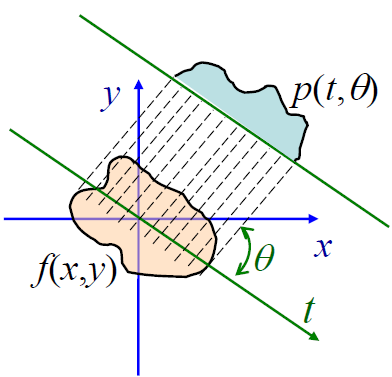
\includegraphics[scale=0.75]{Immagini/radon.png}
\caption{\label{fig:radon} \textit{Oggetto scansionato e sua proiezione}.}
\end{figure}

Dall'insieme delle proiezioni (trasformate di Radon) si ricava il \textbf{sinogramma}. Un sinogramma, mostrato nella \figref{fig:sino}, è un’immagine formata da sinusoidi, ad altezza fissata sul rivelatore, le cui righe rappresentano la proiezione lineare dell'oggetto all'angolo $\theta$; inoltre, deve essere simmetrico rispetto al centro di rotazione e rispetto a rotazioni di 180°. In realtà, l'antitrasformata di Radon vale solamente per variazioni continue di $\theta$, per questo motivo non può essere impiegata nella pratica, dove ovviamente è possibile avere solo variazioni discrete dell'angolo che definisce la direzione di scansione. Si usa, quindi, una versione discretizzata dell'antitrasfornata di Radon.

\begin{figure}[htp]
\centering
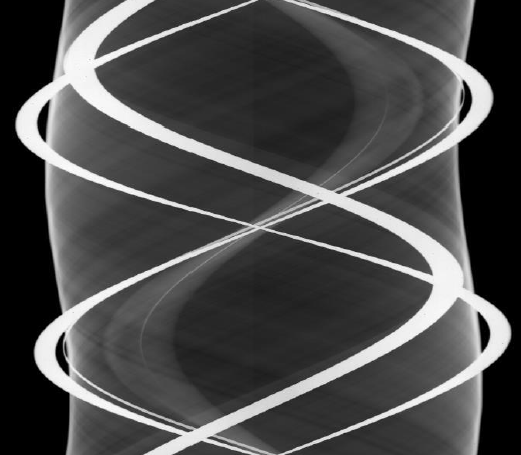
\includegraphics[scale=0.64]{Immagini/sinogramma.png}\quad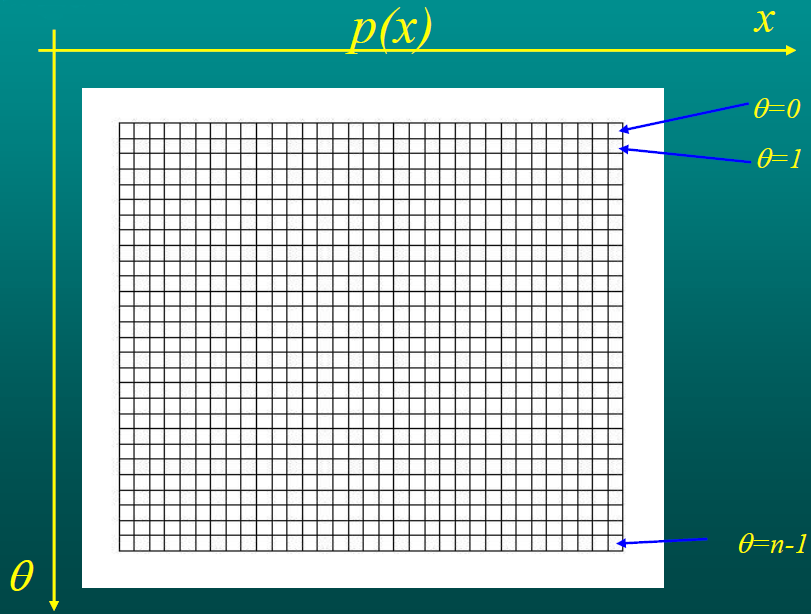
\includegraphics[scale=0.38]{Immagini/sino.png}
\caption{\label{fig:sino} \textit{Sinogramma di un globo e piano di riempimento di un sinogramma}.}
\end{figure}

Una volta che si è acquisito il sinogramma, prima di applicare l'antitrasformata di Radon, per migliorare la qualità dell'immagine (ad esempio rimuovendo rumore o artefatti) è opportuno passare allo spazio delle frequenze. Lo spazio delle frequenze, o spazio di Fourier (\figref{fig:frequenze}), si ottiene applicando al sinogramma la trasformata di Fourier. Se ad ogni proiezione acquisita si applica la trasformata di Fourier, si ottiene una serie di linee nel dominio delle frequenze; tali linee hanno, nel dominio delle frequenze, lo stesso angolo dell'asse \textit{t} corrispondente nello spazio (\textit{x,y}). Questa operazione è conveniente in quanto è molto più semplice operare nello spazio di Fourier per migliorare la qualità dell'immagine, rispetto a quanto non lo sia nello spazio reale utilizzando i \textit{kernel}, come spiegato prima. Una volta che si è migliorata la qualità dell'immagine, si applica l'antitrasformata di Fourier per tornare al sinogramma, e da lì si applica l'antitrasformata di Radon per ottenere l'oggetto.

\begin{figure}[htp]
\centering
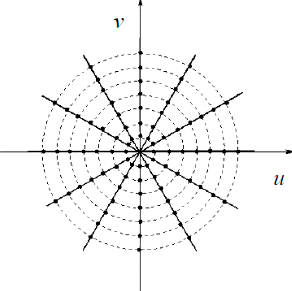
\includegraphics[scale=0.84]{Immagini/frequenze.png}
\caption{\label{fig:frequenze} \textit{Dominio delle frequenze o spazio di Fourier}.}
\end{figure}

L'applicazione dell'antitrasformata di Radon costituisce il processo di \textit{back projection} o retroproiezione. Per capire di cosa si tratta, prendiamo una matrice $3\times3$ di numeri che rappresentano un'immagine, e consideriamo 4 proiezioni, come mostrato nella \figref{fig:proiezione}. Ogni valore proiettato lungo una linea è dato dalla somma dei valori di ciascuna casella della matrice per i quali quella stessa linea passa: questo processo di proiezione è detto \textit{forward projection} e viene eseguito dallo scanner TC in fase di acquisizione. La retroproiezione è il procedimento opposto, in cui lo scanner deve risalire, a partire dalle proiezioni che ha acquisito, al contenuto di ciascuna casella della matrice, che di solito per un'immagine TC è in formato $512\times512$. Nella sua versione più semplice, la retroproiezione viene eseguita semplicemente spalmando il valore delle proiezioni lungo ciascuna linea; tuttavia, questo metodo fornisce risultati non soddisfacenti, in particolare immagini soggette a una caratteristica sfocatura inversamente proporzionale alla distanza dal centro dell'immagine stessa. Per evitare la sfocatura, tra i processi di \textit{forward projection} e \textit{back projection} è necessario filtrare, nello spazio di Fourier, le frequenze che causano la sfocatura e, più in generale, che abbassano la qualità dell'immagine; con questa aggiunta, il processo di retroproiezione prende il nome di \textit{filtered back projection} (FBP). L'impiego delle trasformate e antitraformate di Radon e Fourier è proprio un metodo di FBP.

\begin{figure}[htp]
\centering
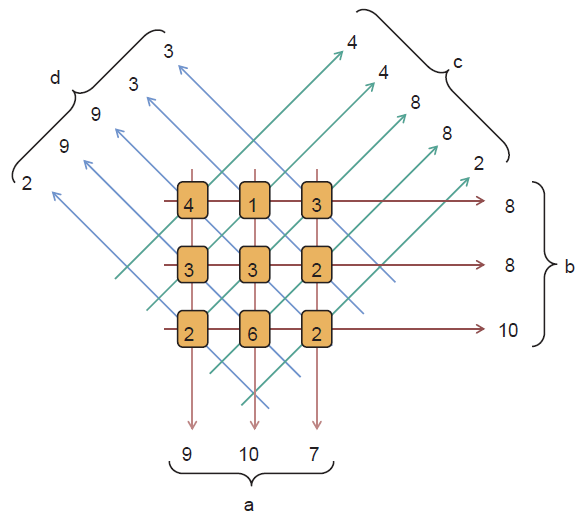
\includegraphics[scale=0.65]{Immagini/proiezione.png}
\caption{\label{fig:proiezione} \textit{Esempio di forward projection per una matrice $3\times3$. Fonte:} \cite[352]{bushberg}.}
\end{figure}

\section{Segmentazione}
Segmentare un’immagine significa riconoscere al suo interno elementi con caratteristiche in comune, distinguere questi elementi da altri con caratteristiche diverse e raggruppare tutti gli elementi simili in regioni, delineando dei bordi tra di esse. In un’immagine digitale, la segmentazione consiste nel classificare e quantificare in qualche modo le proprietà di ciascun pixel, come l’intensità per le immagini monocromatiche, il colore e la \textit{texture}.

Sia \textit{R} l’intera regione di spazio occupata da un’immagine. Possiamo definire la segmentazione di un’immagine come il processo che porta a dividere \textit{R} in sottoregioni $R_i$, con $i = 1,\,\dots,\,n $ tale che:
\begin{enumerate}
\item $\bigcup\limits_{i=1}^n R_i = R$;
\item $R_i$ è un insieme connesso per $i = 1,\,\dots,\,n$;
\item $R_i \cap R_j = \varnothing$;
\item $ \text{Q}(R_k) = 1 $;
\item $ \text{Q}(R_k \cup R_j) = 0 $ per ogni coppia di regioni adiacenti $R_k$ e $R_j$;
\end{enumerate}
dove $\text{Q}(R_k)$ è un predicato logico definito per i punti appartenenti a $R_k$. La condizione 1. asserisce che la segmentazione debba essere completa, nel senso che ogni pixel debba essere incluso in una sottoregione. La condizione 2. richiede che le sottoregioni siano connesse, cioè che non sia possibile individuare al loro interno due o più insiemi aperti, non vuoti e disgiunti. La condizione 3. richiede che le stesse sottoregioni siano disgiunte. La condizione 4. definisce l’assegnazione di un valore booleano a ciascuna sottoregione in base al soddisfacimento di proprietà da definire. Infine, la condizione 5. indica che due sottoregioni adiacenti debbano essere differenti per almeno una proprietà \cite[700]{gonzalez}.

In campo medico, la segmentazione è impiegata per studiare strutture anatomiche, identificare regioni d’interesse dove sono localizzati tumori o lesioni e, cosa più importante per l’obiettivo di questa tesi, misurare il volume dei tessuti corporei. Attualmente nella maggior parte delle strutture sanitarie la segmentazione è effettuata manualmente da un radiologo/radioterapista. La segmentazione manuale dei tessuti corporei è un processo ripetitivo, dispendioso in termini di tempo ed operatore-dipendente: di conseguenza non viene svolto con regolarità su tutte le immagini TC acquisite dai pazienti, sebbene farlo porterebbe a numerosi vantaggi in diversi ambiti. In parecchie strutture, comunque, la segmentazione dei tessuti corporei viene eseguita anche mediante software di segmentazione semiautomatica: si tratta di software che propongono una segmentazione dell'immagine, la quale però necessita di essere comunque controllata e corretta manualmente da un radiologo. Le implicazioni e i vantaggi della segmentazione automatica vengono ampiamente discusse nei capitoli successivi.

Tornando alle basi teoriche della segmentazione, il metodo più semplice è il \textit{thresholding}, in italiano sogliatura, fondato sull'assunto che regioni differenti di un’immagine siano caratterizzate da diversi valori d’intensità. Questo metodo si fonda sul trovare un valore soglia di grigio (\textit{threshold}) tale per cui se un pixel supera quel valore viene considerato un pixel oggetto (\textit{foreground}), mentre se non lo supera viene classificato come pixel di sfondo (\textit{background}) \cite[743]{gonzalez}. Il \textit{thresholding} funziona bene quando sono presenti solo due classi di pixel e se tutti i pixel all’interno di ogni classe hanno intensità simili \cite[20]{LaRosa}; in caso contrario, il metodo da implementare dovrà essere il \textit{multithresholding}, che si fonda sugli stessi principi del \textit{thresholding} ma prevede più di una classe di intensità. Uno dei metodi più famosi di sogliatura è il \textit{thresholding} di Otsu, un algoritmo che trova automaticamente il \textit{threshold}, calcolandolo in modo tale da minimizzare la varianza all'interno di una stessa classe o, equivalentemente, massimizzare la varianza tra le classi. Il metodo di Otsu richiede soltanto l'istogramma di un immagine, ma presenta diverse limitazioni quando il \textit{foreground} e il \textit{background} sono caratterizzati da intensità medie vicine e varianza elevata al loro interno \cite[20]{LaRosa}.

Oltre al \textit{thresholding}, gli algoritmi di segmentazione per immagini monocromatiche funzionano in base a una delle due seguenti proprietà: discontinuità e similarità. L’approccio più comunemente usato per la prima categoria è la segmentazione \textit{edge based}, la quale per funzionare bene necessita che i bordi delle regioni siano sufficientemente diversi l’uno dall'altro e dallo sfondo, in modo da permettere un riconoscimento dei bordi basato sulle discontinuità di intensità locali \cite[700]{gonzalez}. La seconda categoria sfrutta invece la segmentazione \textit{region based}, che consiste nel raccogliere in un gruppo, il \textit{cluster}, pixel con proprietà sufficientemente simili da formare insieme una regione omogenea; il criterio di omogeneità è determinato di solito dal livello di grigio dei pixel \cite{Sharma2010}.

\section{Reti neurali} \label{retineurali}
I recenti software di segmentazione automatica si fondano sul \textit{deep learning}, una branca del \textit{machine learning} basata su reti neurali di algoritmi e che si occupa dei metodi di autoapprendimento per lo svolgimento di compiti complessi. Ciò è possibile grazie alla creazione, in automatico da parte della macchina, di modelli statistici gerarchici, costruiti a partire dalle informazioni più semplici per arrivare alle rappresentazioni più complesse. Ciascuna informazione contenuta in una rappresentazione è chiamata \textit{feature}, o caratteristica; le \textit{feature} create da un umano e fornite alla macchina sono dette \textit{hand crafted feature} \cite[11]{LaRosa}. Più precisamente, una \textit{feature} è una proprietà individuale e misurabile di un fenomeno osservato \cite{bishop, wiki:feature}, solitamente resa in forma numerica \cite{wiki:feature}. Un'importante caratteristica delle reti di \textit{deep learning} è che esse sono costituite da una serie di \textit{layer} successivi: ad ogni \textit{layer}, il segnale in input viene processato e passato al \textit{layer} successivo. I \textit{layer} che si trovano fra l'input e l'output sono definiti nascosti e una rete che abbia questa struttura viene chiamata rete neurale \cite[12]{LaRosa}.

Le reti neurali utilizzate per realizzare gli studi presentati nei capitoli successivi seguono tutte un unico paradigma di apprendimento, l'apprendimento supervisionato. Si tratta di fornire alla rete un insieme di dati di addestramento (\textit{training set}) costituito da oggetti di input e dagli output desiderati, in modo che la rete possa estrarre \textit{feature} significative e trovare una relazione fra l'input e l'output. Successivamente vengono aggiustati i pesi e altri parametri della rete in maniera tale da minimizzare l'errore di previsione relativo al \textit{training set}. Alla fine dell'addestramento, la rete dovrebbe essere in grado di fare delle previsioni, su dati diversi da quelli del \textit{training set}, sull'output desiderato quando questo non è noto a priori \cite{wiki:rete}.

Le reti neurali a convoluzione (CNN), ampiamente utilizzate nei software di segmentazione automatica dei tessuti corporei, sono un tipo di reti neurali artificiali ispirate alla corteccia visuale degli organismi animali, in cui i neuroni sono organizzati in modo da essere sensibili solo a una piccola sottoregione del campo visuale, detta campo ricettivo; i campi ricettivi di tutti i neuroni messi insieme coprono tutto il campo visuale. La convoluzione è la principale operazione matematica impiegata nelle CNN \cite[12]{LaRosa}. La differenza sostanziale fra le CNN e le altre reti neurali artificiali sta nell'organizzazione \virgolette{a griglia} dei dati in input; per questo motivo, le CNN funzionano particolarmente bene quando i dati in input sono delle immagini, che possono essere viste come griglie bidimensionali di pixel. Una qualsiasi CNN è composta da diversi \textit{convolutional} e (eventuali) \textit{pooling layer} alternati, seguiti da uno o più \textit{fully connected layer} prima dell'output. Semplificando, i \textit{convolutional layer} servono ad aumentare le dimensioni dei dati, eseguendo convoluzioni fra un filtro e le immagini 2D: il risultato sarà una mappa d'attivazione per ogni immagine 2D, e tutte le mappe vengono unite insieme per generare un output tridimensionale \cite[13]{LaRosa}. I \textit{pooling layer}, al contrario, servono ad abbassare la dimensione degli input che giungono loro dai \textit{convolutional layer}, prendendo da ciascuna \textit{slice} $2\times2$ soltanto il valore più alto (\textit{max pooling}) o il valore medio (\textit{average pooling}), e mandando questi valori in input al \textit{convolutional layer} successivo \cite{wiki:CNN}. Infine, i \textit{fully connected layer} connettono ogni neurone in un \textit{layer} con ogni neurone in un altro \textit{layer} \cite{wiki:CNN}.

Senza scendere troppo nei particolari della struttura delle CNN, in sostanza queste reti prendono in input un'immagine e restituiscono in output un vettore contenente le probabilità dell'immagine di appartenere a ogni classe prevista: in base a questo, una CNN può essere facilmente adattata per segmentare delle immagini, dove ciascun pixel verrà assegnato a una classe \cite[23]{LaRosa}. Per ridurre il numero di calcoli, il \textit{fully connected layer} può essere sostituito con delle convoluzioni, ma in questo modo l'output della rete risulta di dimensione inferiore all'input; per ovviare a questo problema si possono usare delle operazioni di deconvoluzione, per aumentare la dimensione dell'output fino a che questa abbia raggiunto la stessa dimensione dell'input. Una CNN che non prevede \textit{fully connected layer} nella sua struttura è definita \textit{fully convolutional network} \cite[23-24]{LaRosa}, di cui un importante esempio, nell'ambito della segmentazione automatica, sono le U-Net, chiamate così per la forma a \virgolette{U} che assume la loro schematizzazione, riportata nella \figref{fig:unet}. Il ramo discendente, detto percorso di contrazione (\textit{contracting path}) consiste di due applicazioni ripetute di convoluzioni $3\times3$ e di una operazione di \textit{max pooling} $2\times2$: a ogni \textit{layer}, quindi, la dimensione dell'immagine si dimezza, perdendo informazione spaziale ma aumentando l'informazione sulle \textit{feature}. Al contrario, lungo il ramo ascendente, detto percorso di espansione (\textit{expanding path}), le due applicazioni di convoluzioni $3\times3$ sono seguite da una deconvoluzione $2\times2$, in modo che la dimensione dell'immagine raddoppi a ogni \textit{layer} successivo \cite{wiki:unet}. In questo modo si riacquista l'informazione spaziale persa durante il percorso di contrazione e la si combina con l'informazione sulle \textit{feature} acquisita sempre durate il percorso di contrazione.

\begin{figure}[htp]
\centering
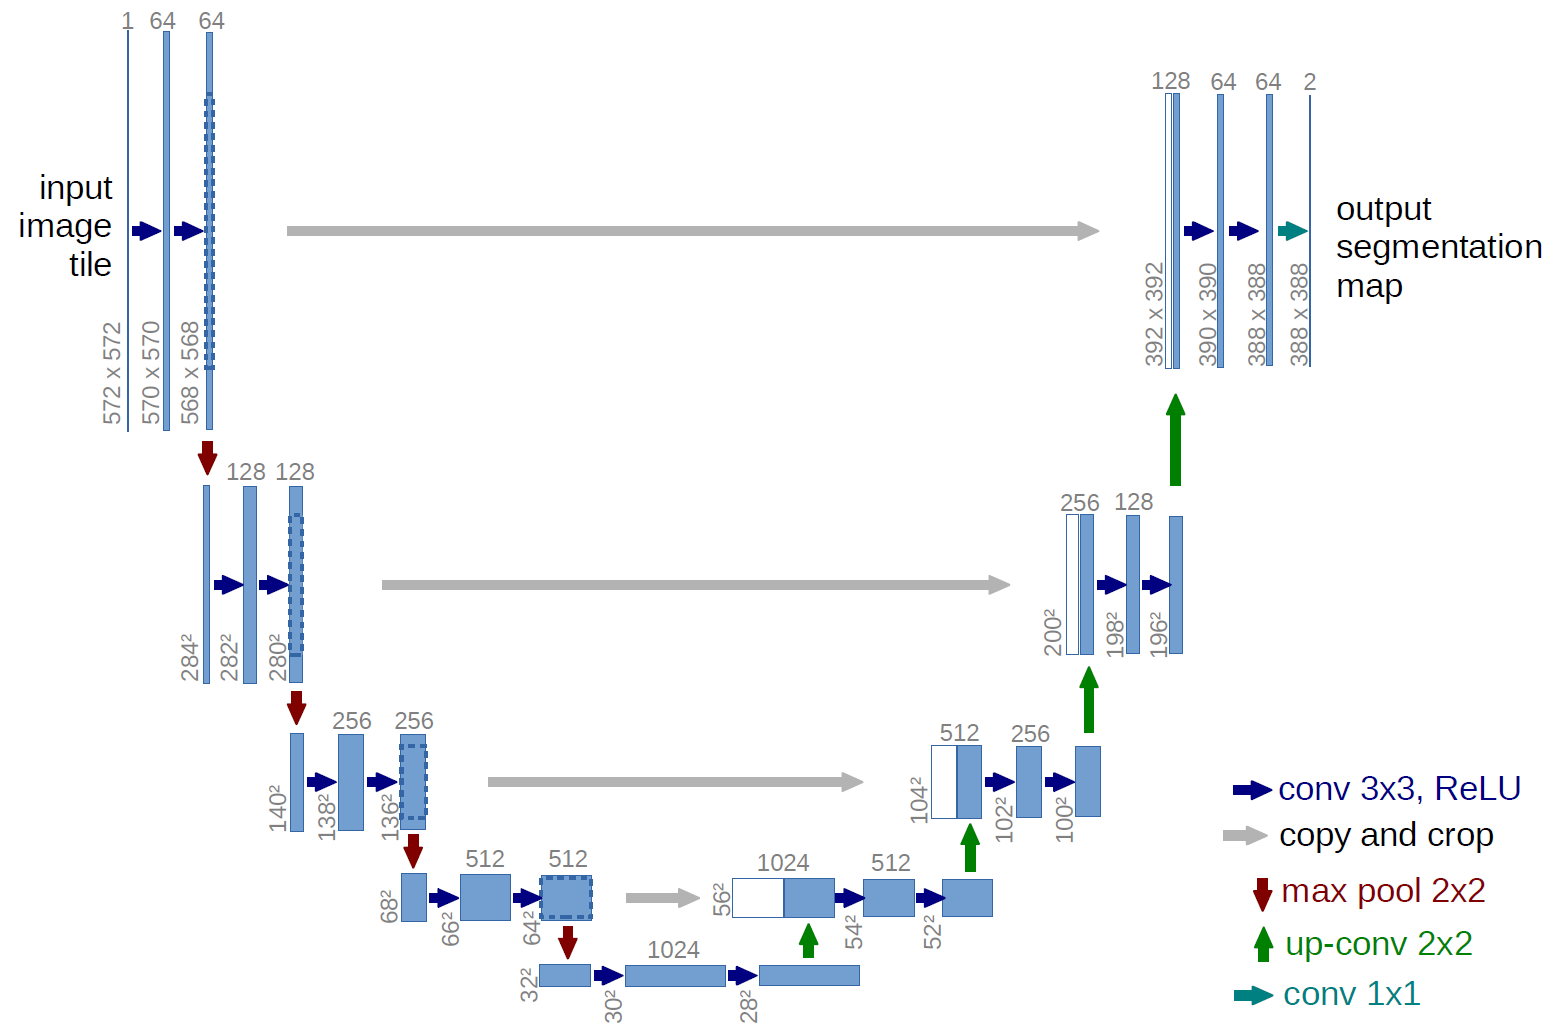
\includegraphics[scale=0.25]{Immagini/unet.png}
\caption{\label{fig:unet} \textit{Schematizzazione di una U-Net}.}
\end{figure}

\section{Metodi statistici per la valutazione della stima della \textit{body composition}}

\subsection{Metodo Kaplan-Meier}\label{km}
In medicina, nei test clinici o comunitari di un determinato farmaco o trattamento, gli effetti della terapia da studiare vengono valutati misurando il numero di soggetti sopravvissuti per un certo periodo di tempo che sono stati sottoposti a quella terapia. Analisi di questo tipo si rivelano spesso complicate per diverse cause: \textit{in primis} alcuni soggetti potrebbero morire durante la finestra di tempo in cui si colloca lo studio ma per cause diverse da quelle studiate, mentre altri ancora non cooperano o smettono di fornire informazioni ai medici sul proprio stato di salute. Per tutti i pazienti per i quali si hanno informazioni parziali si dice che il tempo di sopravvivenza è troncato a destra (\textit{right censored}). Possono esserci anche altri pazienti che si uniscono allo studio dopo il suo inizio, per i quali quindi si ha un tempo di osservazione più breve. Se si vuole tenere conto di tutte queste situazioni, il metodo più semplice è quello di Kaplan-Meier \cite{Goel2010}.

La curva di sopravvivenza di Kaplan-Meier è definita come la probabilità di sopravvivenza in un determinato periodo di tempo, il tempo di sopravvivenza o \textit{serial time}, suddiviso in intervalli più piccoli \cite{altman, Goel2010}. La durata del tempo di sopravvivenza nota di un soggetto è determinata dal verificarsi di un evento di interesse, sia esso la morte del paziente o un altro evento; questo periodo di tempo è noto con il nome di intervallo nell'analisi di Kaplan-Meier ed è rappresentato con una linea orizzontale, come mostrato nella \figref{fig:mm_kaplanmeier}. In altre parole, solo il verificarsi dell'evento di interesse definisce la sopravvivenza nota, mentre i soggetti censurati, rappresentati nella \figref{fig:mm_kaplanmeier} con delle croci, non terminano l'intervallo e quindi non sono associati a nessuno \virgolette{scalino} nel diagramma \cite{Rich2010}. L'analisi di Kaplan-Meier presuppone tre assunzioni:
\begin{itemize}[label=$-$]
    \item ad un qualsiasi istante di tempo i soggetti censurati hanno la stessa aspettative di sopravvivenza dei soggetti di cui si continua ad avere informazioni;
    \item le probabilità di sopravvivenza sono le stesse per tutti i soggetti, a prescindere da quando essi siano stati inclusi nello studio;
    \item qualsiasi evento avviene in un preciso istante di tempo (per eventi su cui si ha incertezza riguardo all'istante di avvenimento, fa fede l'istante al quale l'avvenimento è stato scoperto).
\end{itemize}
Chiaramente, maggiore è la frequenza con la quale vengono acquisite informazioni dai pazienti (sia che riguardino la morte del paziente, sia che riguardino il verificarsi di un evento specifico), maggiore sarà anche l'accuratezza della stima \cite{Goel2010}.

\begin{figure}[htpb]
\centering
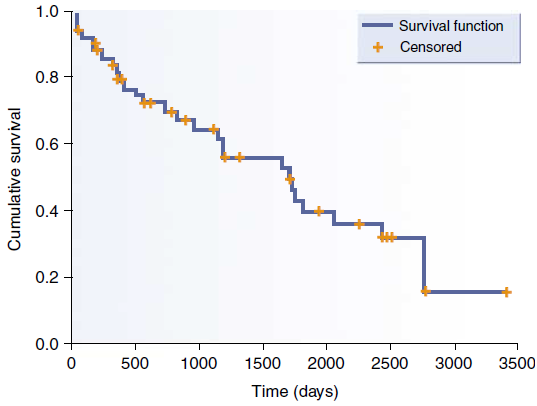
\includegraphics[scale=0.89]{Immagini/mm_kaplanmeier.png}
\caption{\label{fig:mm_kaplanmeier} \textit{Diagramma di Kaplan-Meier della sopravvivenza. Fonte:} \cite{Jager2008}.}
\end{figure}

La sopravvivenza cumulativa mostrata nella \figref{fig:mm_kaplanmeier} è così calcolata: ogni volta che un soggetto X muore, per calcolare la sopravvivenza cumulativa dell'intervallo successivo si prende la frazione di soggetti rimasti in vita subito dopo la morte del soggetto X e la si moltiplica per la sopravvivenza cumulativa dello step precedente, ossia un istante prima che il soggetto X morisse. Si ripete il processo ogni volta che si verifica la morte di un soggetto fino alla fine del periodo di raccolta dati, momento in cui tutti i pazienti rimasti in vita vengono censurati; da questo momento in poi non si hanno più informazioni sui pazienti rimasti in vita, e ognuno di questi potrebbe sopravvivere per diversi anni dopo la fine dell'osservazione con la stessa probabilità con cui potrebbe sopravvivere solo alcune ore, ragion per cui l'estrapolazione dei dati oltre il periodo di osservazione non è giustificata \cite{Rich2010}.

Esistono diversi tipi di curve di sopravvivenza, che si differenziano principalmente per gli eventi d'interesse. Nelle curve di sopravvivenza generale (\textit{overall survival}) l'evento d'interesse è la morte del soggetto per qualsiasi causa, il che fa attribuisce a questo tipo di curva un significato di mortalità piuttosto generale. Nelle curve di \textit{disease free survival} l'evento di interesse è la recidiva di una malattia, mentre le curve di \textit{progression free survival} usano la progressione di una malattia (ad esempio la diffusione di un tumore) come punto finale di un intervallo della curva. Infine, nelle curve di sopravvivenza da malattie specifiche (\textit{disease specific survival}) l'evento di interesse è la morte del soggetto come conseguenza di una malattia specifica; questo tipo di curva può portare a volte a risultati distorti, poiché sarà sempre più alta di curve come quelle di \textit{overall survival} e \textit{disease free survival}, in quanto gli eventi d'interesse sono limitati a una sola malattia specifica \cite{Rich2010}.

\subsection{Modelli di comparazione}\label{confronto}
Un punto importante che rimane da discutere è la comparazione di due curve di sopravvivenza, che torna utile, ad esempio, se si vuole valutare la significatività statistica della differenza fra due curve rappresentanti lo stesso fenomeno ma con cause diverse: ad esempio, la morte di soggetti a causa di insufficienza renale cronica terminale (ESRD) dovuta al diabete o ad altre cause, il cui diagramma di Kaplan-Meier è riportato nella \figref{fig:mm_kaplanmeier2}.

\begin{figure}[htp]
\centering
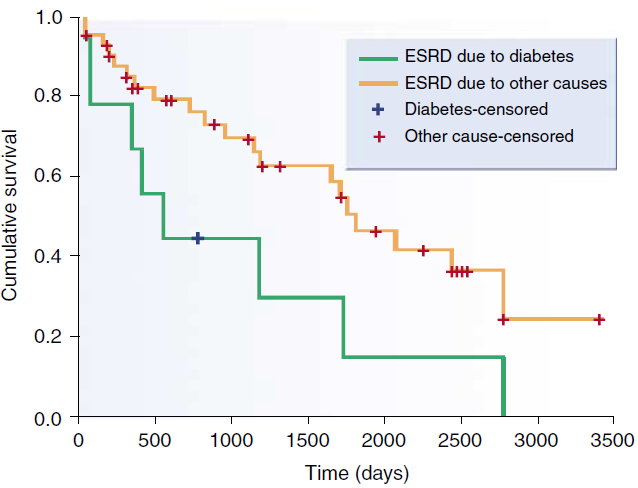
\includegraphics[scale=0.78]{Immagini/mm_kaplanmeier2.png}
\caption{\label{fig:mm_kaplanmeier2} \textit{Diagramma di Kaplan-Meier della sopravvivenza di soggetti estratti da un gruppo a rischio di morte per ESRD dovuta a diabete o ad altre cause. Fonte:} \cite{Jager2008}.}
\end{figure}

Il metodo più comune di comparazione tra due curve di sopravvivenza è il \textit{log-rank test}, che calcola il valore del \textit{chi} quadrato per ogni intervallo di ciascuna curva e li somma tra di loro. Prese due curve di sopravvivenza, siano $E_1$ e $E_2$ i valori di aspettazione del numero di eventi in ciascun gruppo, e siano $O_1$ e $O_2$ il numero totale di eventi osservati in ciascun gruppo. Il \textit{chi} quadrato sarà definito come segue:
\begin{equation}
    \chi^2 = \frac{(O_1-E_1)^2}{E_1} + \frac{(O_2-E_2)^2}{E_2}\,.
\end{equation}
Supponiamo di voler calcolare il valore di aspettazione $E_2$ del numero di eventi del gruppo 2 in un dato intervallo di tempo; questo sarà dato dal prodotto della probabilità dell'evento in entrambi i gruppi 1 e 2 in quell'intervallo (in pratica, la frazione di persone morte dall'inizio alla fine dell'intervallo in entrambe i gruppi) e del numero di persone vive all'inizio dell'intervallo nel solo gruppo 2. Eseguendo questo prodotto per ciascun intervallo del gruppo 2, troviamo il valore di aspettazione totale del gruppo 2. Per trovare il valore di aspettazione totale del gruppo 1, è sufficiente sottrarre al totale degli eventi osservati il valore di aspettazione del gruppo 2 \cite{Goel2010}:
\begin{equation}
    E_1 = (O_1+O_2)-E_2\,.
\end{equation}
Dopo aver ottenuto il $\chi^2$, si controlla il \textit{p-value} all'interno della tavola del \textit{chi} quadrato per un solo grado di libertà e si stabilisce la significatività della differenza fra i due gruppi se il \textit{p-value} è minore di un certo valore stabilito a priori.

Il \textit{log-rank test} permette unicamente di stabilire la significatività statistica della differenza fra le curve di sopravvivenza di due gruppi, perciò è utile solo in analisi univariate. Per lo svolgimento di analisi multivariate nel campo delle curve di sopravvivenza, il metodo più diffuso è il modello di regressione di Cox (\textit{Cox proportional hazards model}), che permette di testare l'effetto di altre variabili indipendenti sui tempi di sopravvivenza dei diversi gruppi \cite{Goel2010}, ad esempio per lo studio del rapporto tra un fattore di rischio (come il fumo) e l’incidenza di un determinato esito clinico (come l'infarto del miocardio), correggendo per uno o più fattori di confondimento (quali l’obesità e l’ipertensione) \cite{Provenzano2013}. Il rischio (\textit{hazard}) costituisce la variabile dipendente ed è definito come la probabilità di morte ad un certo istante \cite{Goel2010}; in altre parole, è il tasso di incidenza di un evento d'interesse, cioè il numero di eventi per persona per unità di tempo \cite{Provenzano2013}. Il rapporto di rischio, invece, è il rapporto tra i tassi di rischio istantanei di un evento d'interesse in due gruppi diversi \cite{wiki:rischio}: per fare un esempio, se $H_1,\,H_2,\,H_3,\,\dots$ e $h_1,\,h_2,\,h_3,\,\dots$ sono i tassi di rischio per due gruppi agli istanti $T_1,\,T_2,\,T_3,\,\dots$, i rapporti di rischio agli istanti $T_1,\,T_2,\,T_3,\,\dots$ saranno rispettivamente $\frac{H_1}{h_1},\,\frac{H_2}{h_2},\,\frac{H_3}{h_3}\,,\dots$. Si assume che il tasso di rischio rimanga costante nel tempo, ossia che $\frac{H_1}{h_1}=\frac{H_2}{h_2}=\frac{H_3}{h_3}=\dots$ \cite{Goel2010}.

L’equazione generale di un modello di regressione di Cox avente
l’obiettivo di analizzare il rapporto tra la presenza/assenza di un singolo
fattore di rischio e un determinato esito clinico è la seguente:
\begin{equation}\label{rischio}
    h_i(t) = \lambda_0(t)\,\mathrm{e}^{\beta_1 x_i}\,,
\end{equation}
dove $h_i(t)$ è il tasso di incidenza stimato dell'evento al tempo \textit{t}, $\lambda_0(t)$ rappresenta il rischio di base, cioè il tasso di incidenza dell'evento in assenza del fattore di rischio, $\beta_1$ è il coefficiente di regressione e $x_i$ è il fattore di rischio considerato. Applicando il logaritmo naturale all'\eqref{rischio}, si ottiene:
\begin{equation}
    \ln{(h_i(t))} = \ln{(\lambda_0(t))} + \beta_1 x_i = \beta_0(t) + \beta_1 x_i\,;
\end{equation}
in questa forma, l'equazione sembra più simile a una classica equazione di regressione lineare \cite{Goel2010, vanDijk2008}.

\subsection{Metodo Bland-Altman}\label{blandaltman}
I metodi di correlazione sono strumenti statistici che rivelano in che misura delle coppie di variabili sono correlate. Il risultato principale di una correlazione è il coefficiente di correlazione \textit{r}, che può variare da $-1$ a $+1$, e più si avvicina agli estremi, più le variabili saranno correlate. Tuttavia, le tecniche di correlazione descrivono solamente la relazione fra due insiemi di dati, non il loro accordo \cite{Udovicic2007,Giavarina2015}, risultando a volte inadeguate e foriere di risultati ambigui.

Il metodo Bland-Altman è uno strumento molto efficace per la valutazione dell'accordo fra due metodi di misurazione, consentendo inoltre di individuare la presenza di differenza sistematiche, valori anomali (\textit{outlier}) e particolari strutture di disaccordo (\textit{pattern}) \cite[357]{szklo,Franco2017}. In breve, il metodo quantifica il livello di accordo tra due misure mediante la definizione di due limiti di concordanza mostrati su uno \textit{scatter plot}: sull'asse delle ordinate viene posta la differenza fra due misure in una stessa coppia (che possono essere, ad esempio, due misure di pressione arteriosa effettuate su uno stesso soggetto con due metodi diversi), mentre sull'asse delle ascisse è riportato il valore medio delle due misure in una stessa. In un diagramma di Bland-Altman, di cui si riporta un esempio nella \figref{fig:ba}, sono presenti due elementi fondamentali:
\begin{itemize}[label=$-$]
    \item il \textit{bias}, cioè una linea appresentante la media delle differenze delle due misurazioni;
    \item i limiti di concordanza, due linee che vengono tracciate ad altezza $bias\,\pm\,1,96\,\sigma$, dove $\sigma$ è la deviazione standard.
\end{itemize}

Nel caso in cui la prima e la seconda misurazione fossero coincidenti, la media delle differenze sarebbe nulla e i punti sarebbero allineati lungo l’asse delle ascisse sul valore 0. La scelta di rappresentare in ascissa la media delle due misurazioni, al posto dei valori di una sola delle due misurazioni, si basa sul fatto di non conoscere a priori il valore vero della variabile in
esame; di conseguenza, si prende in considerazione la migliore stima, che è rappresentata dalla media \cite{Franco2017}.

Il valore di $1,96\,\sigma$ rispetto alla media (spesso approssimato a $2\,\sigma$) utilizzato come limite di concordanza è dovuto al fatto che, se le differenze fra le misure sono distribuite normalmente, queste devono essere contenute per il 95\% del totale tra i due limiti così definiti. Non è necessario che le misure seguano una distribuzione normale \cite{BlandAltman}, mentre se le differenze non seguono una distribuzione normale, si può provare ad eseguire una trasformazione logaritmica dei dati originali per provare a normalizzare la distribuzione delle differenze \cite{Giavarina2015}.

Infine, per valutare se i dati forniti dai due metodi di misura abbiano un livello di accordo sufficiente, l'unico modo è confrontarli con limiti di accettabilità definiti a priori in base a criteri clinici e analitici: se i limiti di concordanza trovati con l'analisi di Bland-Altman cadono all'interno dei limiti di accettabilità, allora consideriamo i due insiemi di dati sufficientemente concordi \cite{Giavarina2015}. Nel caso si confrontino un metodo di misura \textit{gold standard} e un metodo di misura, una buona regola pratica è quella di considerare come \textit{bias} accettabile un valore non superiore del 3-4\% rispetto a quello fornito dal dispositivo \textit{gold standard} \cite{Weinfurt2010,Franco2017}.

\begin{figure}[htp]
\centering
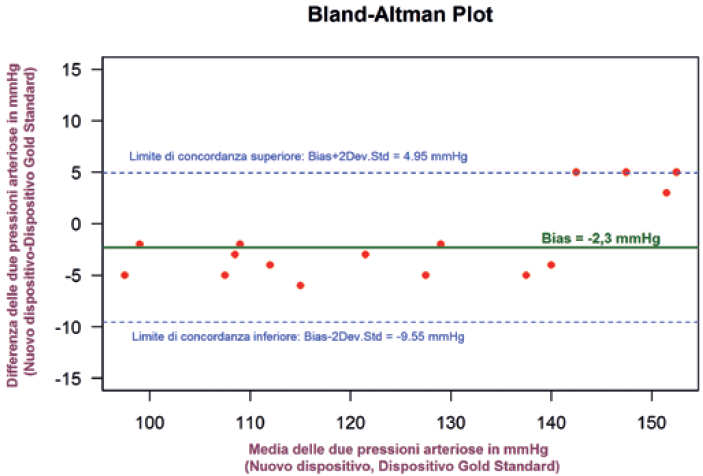
\includegraphics[scale=0.8]{Immagini/ba.png}
\caption{\label{fig:ba} \textit{Grafico di Bland-Altman dell'accordo nelle misurazioni della pressione diastolica con due dispositivi: il gold standard e il nuovo
dispositivo. Si può notare che per valori di pressione media superiori a $140\,\mathrm{mmHg}$ il nuovo dispositivo fornisce misure non concordanti con quelle del gold standard. Fonte:} \cite{Franco2017}.}
\end{figure}